%----------------------------------------------------------------------------------------
%	CHAPTER 2
%----------------------------------------------------------------------------------------
\chapterimage{chapter_head_math.pdf} % Chapter heading image

\chapter{Estágios do ciclo da aprendizagem}
\label{cap:aprendizagem}




\section{Estágios da aprendizagem}
\label{sec:aprendizagem}

Quando desejamos apreender uma nova habilidade ou conhecimento, já seja tocar o piano,
resolver problemas matemáticos,
jogar futebol, ou dançar; devemos atravessar por um processo de aprendizagem dividido em estágios;
o conhecimento destes estágios nos permitirá modelar melhores estrategias e exercícios para o aprendizado,
focando-nos no estagio em que se encontre cada pessoa.

De acordo com a programação neuro linguística (PNL), 
entre os estágios do processo (ciclo) de aprendizagem podemos achar:
a incompetência inconsciente, a incompetência consciente, 
a competência consciente e finalmente a competência inconsciente 
\cite[pp. 249]{seymourtreinando} \cite[pp. 10]{passadori7} \cite{de2013treinamentos};
ver Tabela \ref{tab:learning1}.

\begin{table}[!h]
  \centering
  \begin{tabular}{|l||l|l|}
   \hline
    ~             & incompetência & competência \\ \hline \hline
    inconsciente  & Estágio 1     & Estágio 4   \\ \hline
    consciente    & Estágio 2     & Estágio 3   \\ \hline
  \end{tabular}
  \caption{Estágios da aprendizagem.}
  \label{tab:learning1}
\end{table}

\begin{description}
%%%%%
\item[incompetência inconsciente:] Neste estágio da aprendizagem não temos consciência do que devemos fazer ou aprender,
e consequentemente temos incompetência na área que desejamos desenvolve-nos e/ou vivemos numa ``alegre ignorância'';
``você não sabe o que não sabe'' \cite[pp. 29, 252]{seymourtreinando} \cite{carnegie2014lideranca} \cite{de2013treinamentos}.
Existe a possibilidade que ao desconhecer nossas próprias limitações,
tendamos achar que o problema da falta de sucesso é externo a nós \cite[pp. 10]{passadori7}.
%%%%%
\item[incompetência consciente:] Neste estágio você sabe o que deve fazer ou aprender,
\label{ref:IncompetenciaConsciente}
porem não consegue realizar a tarefa de forma competente;
por este motivo a tarefa exige toda nossa atenção, 
este estágio da aprendizagem pode trazer algum desconforto,
mas a taxa de aprendizagem é maior neste estágio;
``você descobre o que não sabe, consequentemente, descobre uma incompetência nesse ponto''
\cite[pp. 29]{seymourtreinando} \cite{carnegie2014lideranca} \cite[pp. 10, 11]{passadori7} \cite{de2013treinamentos}.
%%%%%
\item[competência consciente:] 
\label{ref:CompetenciaConsciente}
Neste estagio somos competentes, 
porem precisamos de toda nossa atenção consciente 
para realizar uma determinada tarefa; a tarefa ainda não tem-se tornado um hábito em nós 
\cite[pp. 30, 249]{seymourtreinando} \cite{carnegie2014lideranca} \cite{de2013treinamentos}.
Esta é a fase do condicionamento positivo,
onde a pessoa deve estar em exercício continuo com reforços positivos para fixar o aprendizado \cite[pp. 11]{passadori7}.
%%%%%
\item[competência inconsciente:] 
\label{ref:CompetenciaInconsciente}
Neste estágio a habilidade em estudo tem sido plenamente integrada em nós, 
e podemos realizá-la sem esforço, de forma inconsciente, com confiança e naturalidade, 
de modo que podemos realizar outras atividades em paralelo;
``maestria intuitiva e instintiva'' \cite[pp. 30, 249]{seymourtreinando} \cite[pp. 11]{passadori7} \cite{de2013treinamentos}.
\end{description}


\begin{elaboracion}[title=O cerebelo e o comportamento inconsciente, width= 1.00\linewidth]
%   https://books.google.com.br/books?id=cf3AAdIH1UQC&pg=PA35&dq=compet%C3%AAncia+inconsciente+cerebelo&hl=pt-BR&sa=X&ved=0ahUKEwir6qfn4OzkAhVzKLkGHTvZD1wQ6AEIUzAF#v=onepage&q=compet%C3%AAncia%20inconsciente%20cerebelo&f=false
O cerebelo (``cérebro pequeno'' em latim) é uma protuberância ampla e convoluta,
localizada na fossa posterior do crânio, 
e está conectada à parte traseira do tronco encefálico \cite[pp. 93]{gazzanigaciencia} \cite[pp. 87]{carneiro2004atlas}
\cite[pp. 516]{bearneurociencias}.

A função mais evidente do cerebelo é a aprendizagem motora e a memoria motora,
sendo o grande coordenador da ação muscular ``inconsciente'';
ao contrario do cérebro que atua de forma ``consciente'' 
\cite[pp. 93]{gazzanigaciencia} \cite[pp. 87]{carneiro2004atlas} \cite[pp. 516]{bearneurociencias}.

O cerebelo é quem nos permite estar caminhado de forma inconsciente,
e ao mesmo tempo poder raciocinar uma fala com alguém ou planejar nosso dia de trabalho.
\end{elaboracion}



\section{Ciclo da aprendizagem - PDCA}
\label{sec:cicloaprendizagem}
O ciclo que seguimos para potencializar nossa aprendizagem \cite[pp. 13]{mumford2001aprendendo},
em muitos aspectos se parece ao ciclo, para a melhoria continua, na gerencia de projetos 
\cite[pp. 4]{caloba2018gerenciamento} \cite[pp. 59]{teixeira2018gestao}.
Na literatura, este é conhecido como ``ciclo PDCA'';
a sigla vem das palavras em inglês: ``Plan'', ``Do'', ``Check'' e ``Act'';
estas podem ser interpretadas como: Planejar, fazer, verificar e atuar em consequência
\cite[pp. 59]{teixeira2018gestao} \cite[pp. 4]{caloba2018gerenciamento}.
Este fluxo de trabalho, também é chamado ``ciclo de Shewhart'' em honor a seu inventor,
ou ``ciclo de Demming'' em honor a um de seus grandes difusores no Japão
\cite[pp. 59]{teixeira2018gestao} \cite[pp. 4]{caloba2018gerenciamento}.

A Figura \ref{fig:ciclopdca} mostra em detalhe o fluxo de trabalho no ciclo PDCA.
\begin{figure}[!h]
  \centering
\smartdiagram[circular diagram:clockwise]{Fazer, Verificar, Atuar, Planejar}
    %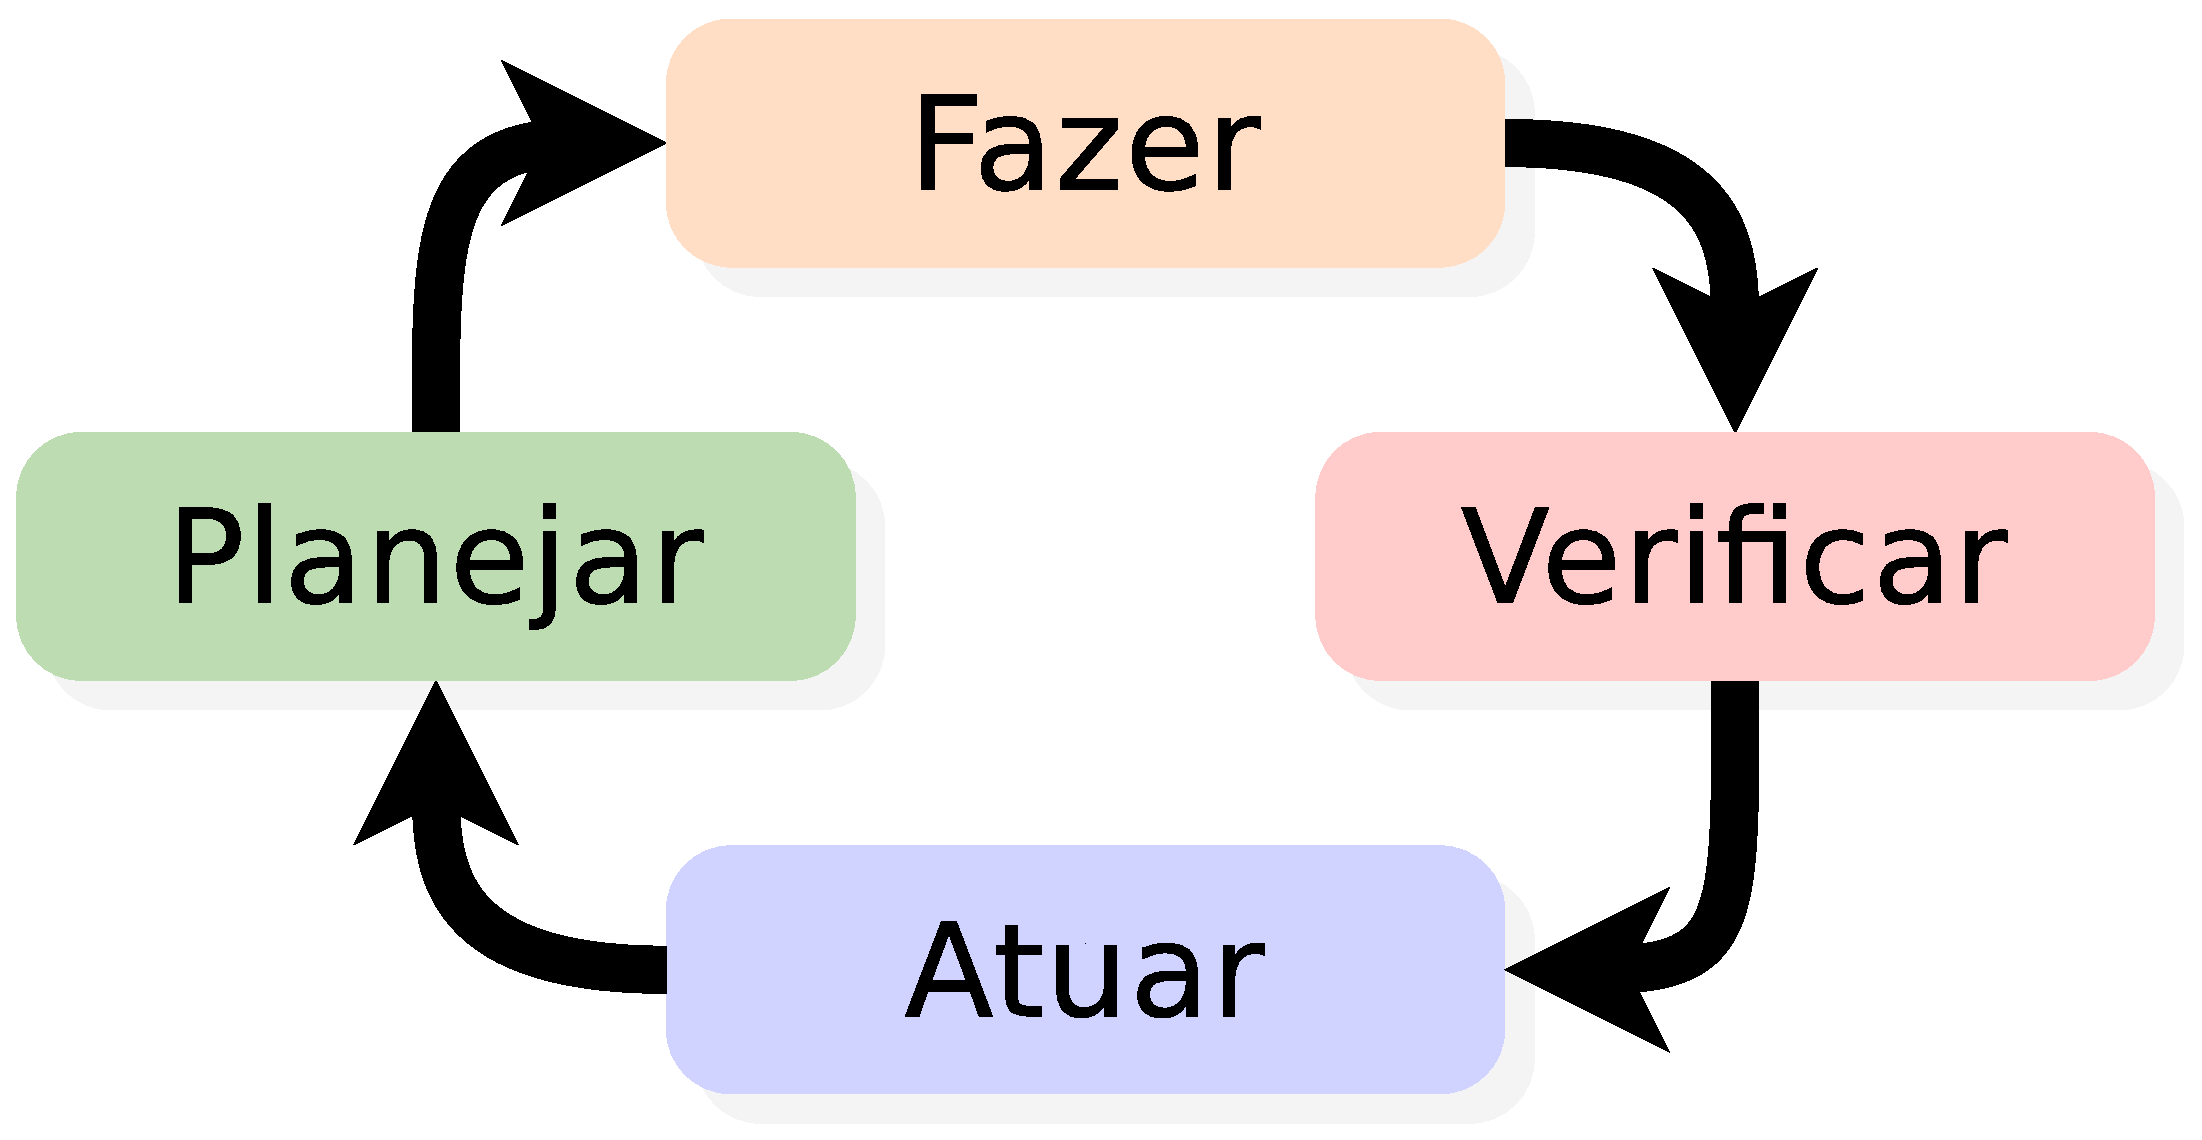
\includegraphics[width=0.55\textwidth]{chapters/cap-learning/ciclo2.eps}
\caption{Ciclo PDCA.}
\label{fig:ciclopdca}
\end{figure}

\begin{description}
\item[Planejar:] Estabelecemos nosso objetivo no aprendizado; 
realizamos um planejamento do caminho que seguiremos para atingir nossos objetivos.
\item[Fazer, desenvolver:] Pomos em prática o trabalho anteriormente planejado;
coletamos dados sobre nosso desenvolvimento nas tarefas escolhidas.
\item[Verificar, conferir:] Comparamos o resultado obtido com o esperado;
realizamos uma avaliação de nosso despenho e competência.
\item[Atuar, agir, ajustar:] Tomamos ações corretivas no nosso plano de trabalho,
para diminuir as diferenças entre o resultado obtido e o esperado.
\end{description}


\begin{tcbattention}
Uma pessoa inteligente aprende do seus próprios erros,
uma pessoa sabia aprende dos erros dos demais.
\begin{flushright}
Fernando P. R.
\end{flushright}
\end{tcbattention}


\section{Percepção e aprendizagem}
\label{sec:percepcionaprendizagem}

O ser humano entende o mundo que lhe rodeia mediante o uso do seus sentidos,
de modo que suas percepções podem ser de caráter \cite[pp. 28]{ready2010pnl}:
\begin{itemize}
\item visual (olhos), 
\item auditivo (ouvidos),
\item cinestésico (emoções e tato), 
\item olfativo (nariz) e
\item gustativo (gusto).
\end{itemize}
Entre todas estas possíveis fontes de informação,
pelo geral, quando estamos em nosso momento de maior estresse,
cada um de nós manifestamos preferencia por alguma destas 5 fontes de informação;
este sentido preferenciado é conhecido como ``sistema figurativo'' ou ``representação primordial''
\cite[pp. 28]{ready2010pnl}.

Seja metafórica ou real nossa fonte de conflito, o estresse sempre estará presente,
e nosso corpo acude a nossa representação primordial para obter informação.
Quando tentamos alcançar a competência numa área desfavorável para nós\footnote{Estágio 
2 de nosso aprendizado visto na Pag. \pageref{ref:IncompetenciaConsciente}.},
podemos atingir o estresse, consequentemente nosso corpo acudirá com atenção a 
nossa representação primordial;
pelo que é interessante fazer um exame de autoconhecimento, 
para poder saber qual é este sentido em nós e assim otimizar nosso processo de aprendizagem.


% https://books.google.com.br/books?id=zxYIsvdXo_QC&pg=PA137&dq=modo+de+aprender+cinest%C3%A9sico&hl=pt-BR&sa=X&ved=0ahUKEwi1lJGkye7kAhWvH7kGHb2TCOoQ6AEILzAB#v=onepage&q=cinest%C3%A9sico&f=false
% https://books.google.com.br/books?id=ioi2Ic-FRWUC&pg=PA152&dq=visual+auditivo+cinest%C3%A9sico&hl=pt-BR&sa=X&ved=0ahUKEwjwou29ye7kAhU-IbkGHVpBAI0Q6AEIOTAD#v=onepage&q=visual%20auditivo%20cinest%C3%A9sico&f=false


\begin{elaboracion}[title=Ditado chines, width= 1.00\linewidth]
Existe um velho ditado chines atribuído a Confúcio \cite[pp. 60, 63]{AprendendoInteligencia2008} \cite[pp. 9]{abe2002introducao}:\\
\begin{center}
    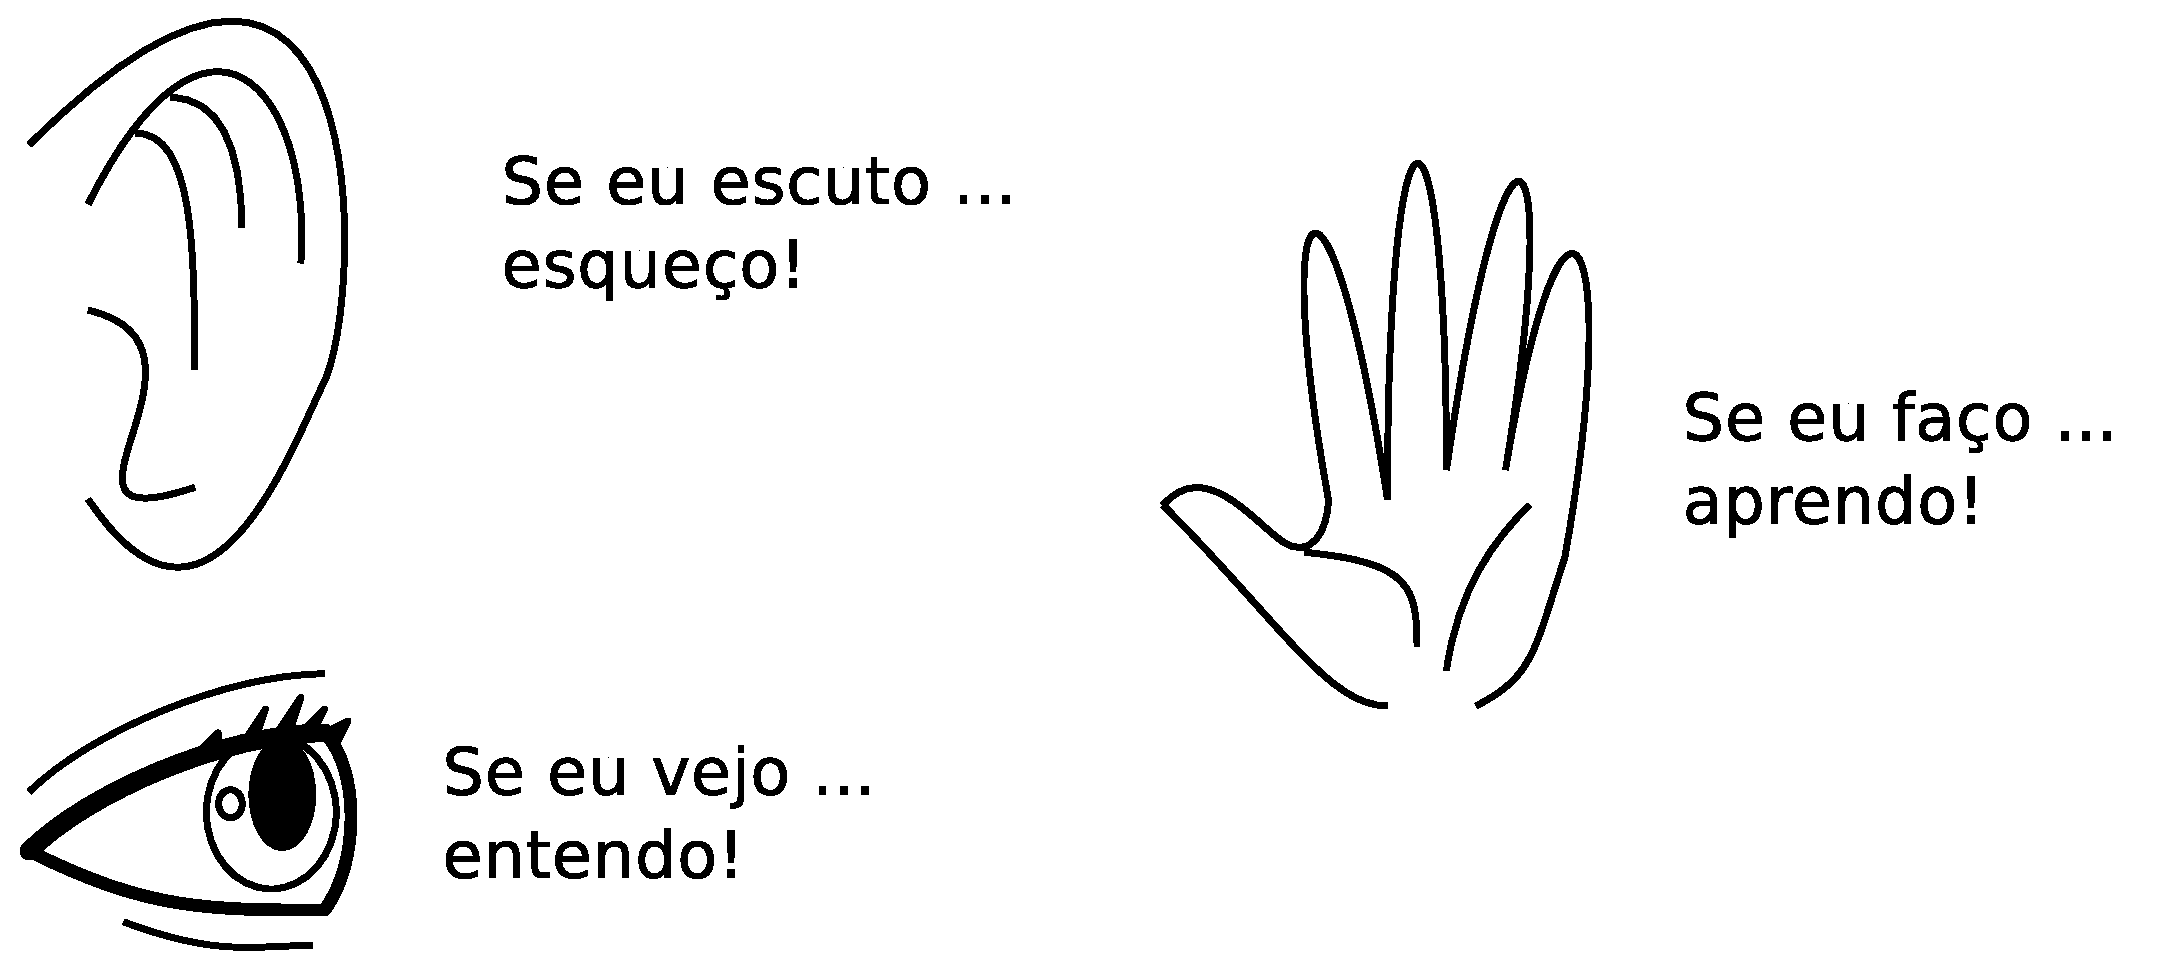
\includegraphics[width=0.8\textwidth]{chapters/cap-learning/ditadochines.eps}
\end{center}
\end{elaboracion}
